\chapter{Automatización de cajeros automáticos}
En este capítulo, se analizó y modeló un proceso asignado por un colaborador del banco de Bogotá, el modelado del proceso se hizo usando el estándar BPMN definido en el capítulo ~\ref{ch:BPMN}.

\section{Descripción del proceso (Automatización de cajeros automáticos)}
Desde un área de Canales Electrónicos del banco de Bogotá surgió una iniciativa para automatizar el proceso de informar sobre el estado de los cajeros automáticos del Banco de Bogotá, donde cualquier colaborador puede reportar las fallas que encuentre en los cajeros automáticos usando un formulario que activa un flujo de Power Automate que requiere el código o la dirección específica del cajero en cuestión. Cuando un colaborador del banco encuentra un cajero con una falla, este tiene la posibilidad de informar al área encargada de esta falla, dependiendo de la región la falla se le notifica a una persona en específico para que gestione y repare la falla del cajero.

Modelo resultante (figura ~\ref{fig:AcA}).

\begin{figure}[H]
	\centering
	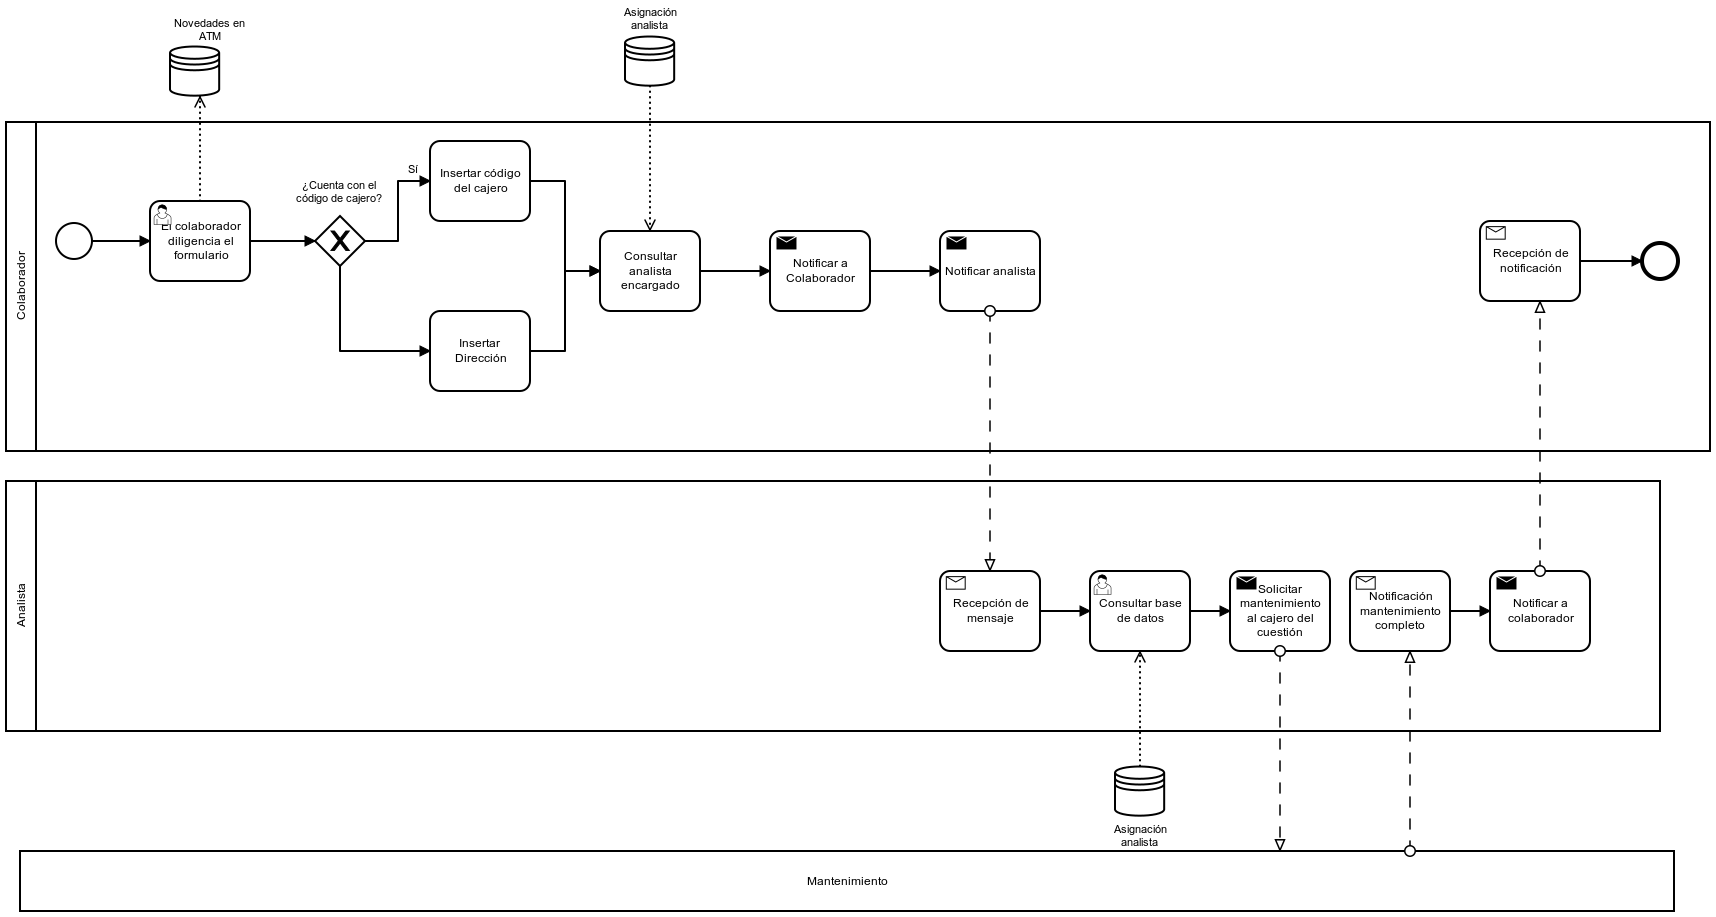
\includegraphics[scale=0.25]{Capitulo3/imagenes/diagram-Cajeros.png}
	\caption{Automatización de cajeros automáticos}
	\label{fig:AcA}
\end{figure}

\section{Construcción del modelo}

\subsection{Participantes}
Dentro de la descripción se pudieron identificar los siguientes participantes: 
\begin{itemize}
	\item \textbf{Colaborador: }Es el colaborador que inicia el flujo al  solicitar mantenimiento del cajero automático.
	\item \textbf{Analista: } Es la persona encargada de darle solución al caso.
	\item \textbf{Mantenimiento: } Es un participante del proceso que interfiere directamente en el proceso al hacerle mantenimiento a los cajeros.
\end{itemize}

Ya con los participantes identificados se da inicio al proceso usando un evento de inicio básico, cuando el colaborador está haciendo la solicitud tiene la opción de notificar la falla del cajero e identificarlo por la dirección en la cual está ubicado el cajero o por un código único que los identifica.

\begin{figure}[H]
	\centering
	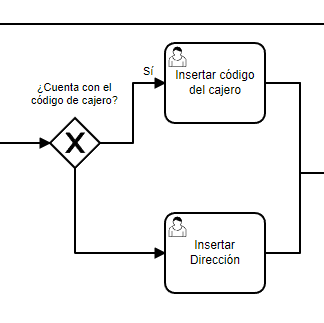
\includegraphics[scale=0.5]{Capitulo3/imagenes/1.png}
	\caption{¿Cuenta con el código del cajero?}
	\label{CodCaj}
\end{figure}

El proceso debe consultar a que analista le corresponde el cajero (Por zona se tiene un analista asignado), se consulta en la base de datos el analista al que se debe notificar, también se le notifica al colaborador que su solicitud fue recibida y este está enterado.

\begin{figure}[H]
	\centering
	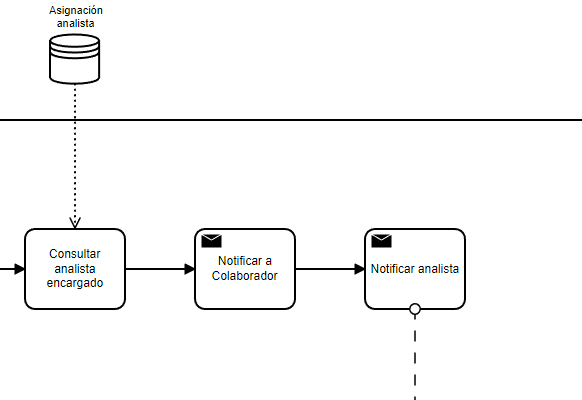
\includegraphics[scale=0.5]{Capitulo3/imagenes/2.png}
	\caption{¿Cuenta con el código del cajero?}
	\label{CodCaj2}
\end{figure}

Cuando el analista recibe la notificación debe hacer la gestión con el participante encargado del mantenimiento, el analista debe hacer la solicitud a mantenimiento y esperar que este le notifique que el mantenimiento está completo.

\begin{figure}[H]
	\centering
	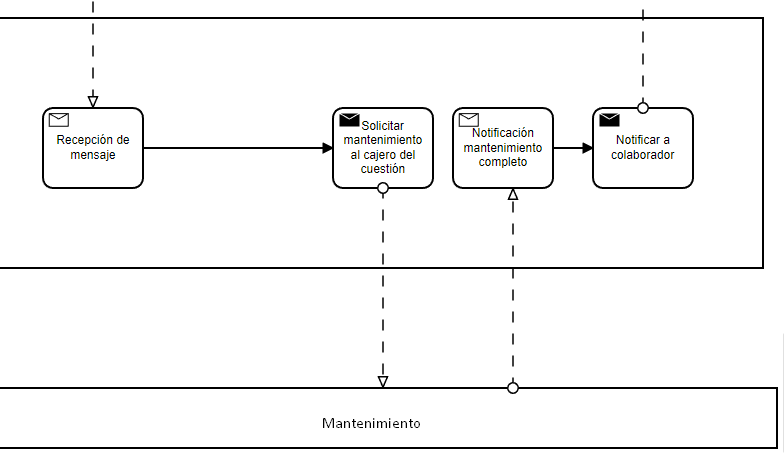
\includegraphics[scale=0.5]{Capitulo3/imagenes/3.png}
	\caption{Notificaciones}
	\label{notificaciones}
\end{figure}

Seguido se notifica al colaborador que se le dio solución al caso y se cierra el proceso.
\begin{figure}[H]
	\centering
	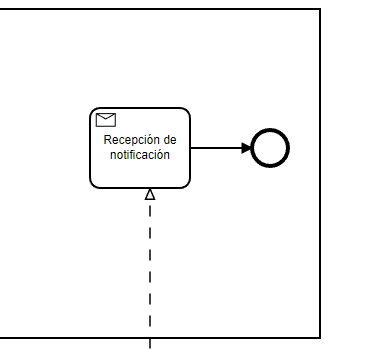
\includegraphics[scale=0.5]{Capitulo3/imagenes/4.png}
	\caption{Final del proceso}
	\label{Finproceso}
\end{figure}

\section{Implementación}
\subsection{Lista en SharePoint}\label{listasSp}
La lista de SharePoint es la herramienta que se usa dentro de la organización para coleccionar y organizar datos que se usan o consumen los flujos de Power Automate, la estructura de la lista así como los tipos de columna se hicieron acorde a la solicitud del colaborador de Canales electrónicos
.
\subsubsection{Lista Novedades en ATM}
\begin{figure}[H]
	\centering
	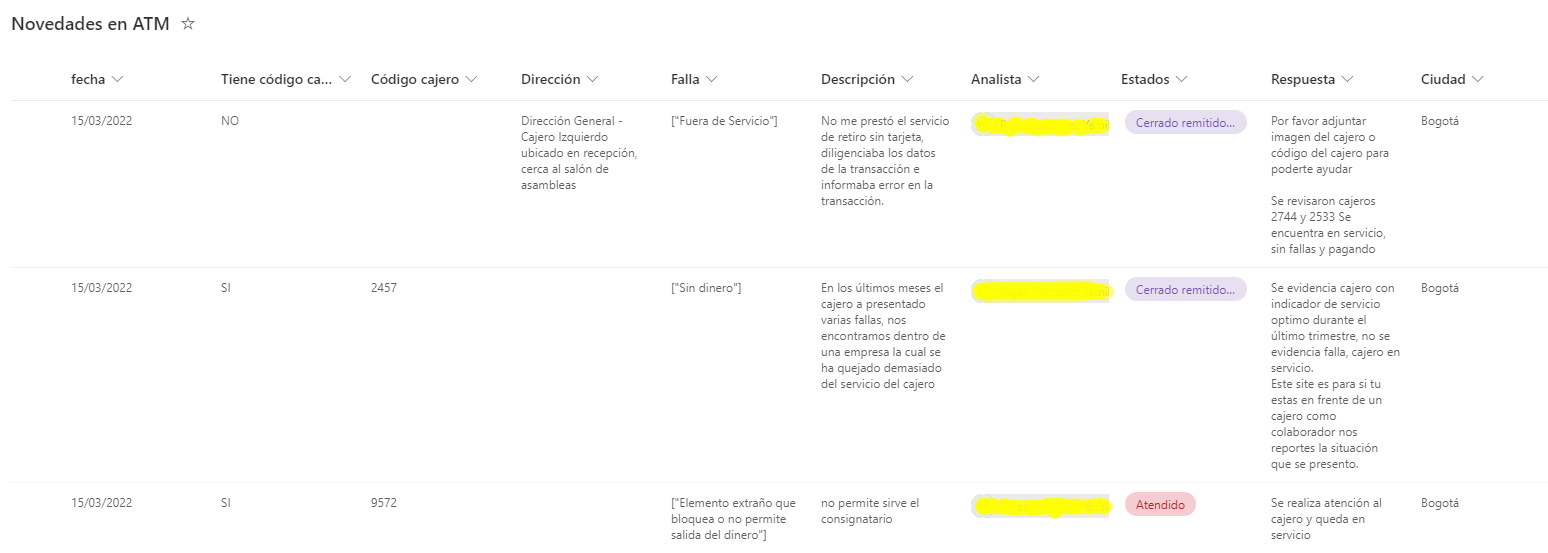
\includegraphics[scale=0.37]{Capitulo3/imagenes/6.png}
	\caption{Oficinas Novedades en ATM}
	\label{ListaNovedadesEnATM}
\end{figure}

\subsubsection{Lista Novedades en ATM}
\begin{figure}[H]
	\centering
	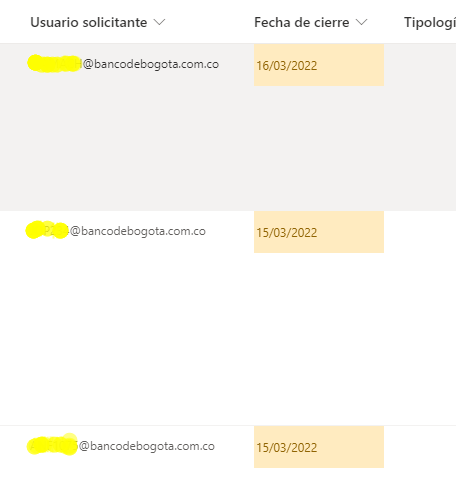
\includegraphics[scale=0.37]{Capitulo3/imagenes/7.png}
	\caption{Oficinas Novedades en ATM}
	\label{ListaNovedadesEnATM2}
\end{figure}

Las columnas se configuraron de la siguiente manera.

\begin{itemize}
	\item \textbf{ID: }Es una columna numérica única autoincrementable que define SharePoint de manera automática.
	\item \textbf{Fecha: } Esta columna toma valores dependiendo de la fecha de cierre del caso, esta columna se configuró como ``Fecha''.
	\item \textbf{Tiene código cajero: }Esta columna almacenará valores de tipo booleano (true o false), dependiendo si tiene o no el código de cajero a reportar.
	\item \textbf{Código cajero: }Es una columna numérica que almacena los códigos de los cajeros, es un número de cuatro dígitos, esta columna se definió de tipo ``Número''.
	\item \textbf{Dirección: } Es un valor alfabético o alfanumérico que define el nombre de una oficina, por este motivo se definió el tipo de la 
	columna como ``Una sola línea de texto''.
	\item \textbf{Falla: }Es un valor alfabético donde almacenamos la falla del cajero (Sin dinero, Falla en la lectura de la trajeta, etc), por este motivo definimos el tipo de la columna como ``Una sola línea de texto''.
	\item \textbf{Descripción: } Es un valor de tipo alfabético, pero debido a que el número de caracteres puede ser muy grande se define ``Varias líneas de texto'' debido a la capacidad que tienen de almacenar mayor cantidad de número de caracteres.
	\item \textbf{Analista: } Esta columna almacenará un objeto con los atributos (Nombre, Email, Cargo, etc.) del colaborador al cual se le asigne la solicitud, esta columna se configuró de tipo ``Usuario''.
	\item \textbf{Estados: }Esta columna almacena una serie de valores permitidos (Abierto, En trámite, Vencido, Cerrado, remitido erradamente, Atendido) pero solamente puede tomar uno de estos valores, esta columna se definió de tipo opción.
	\item \textbf{Respuesta: } Es un valor de tipo alfabético, pero debido a que el número de caracteres puede ser muy grande se define ``Varias líneas de texto'' debido a la capacidad que tienen de almacenar mayor cantidad de número de caracteres.
	\item \textbf{Ciudad: } Esta columna toma valores dependiendo de la ubicación del cajero, esta columna se configuró como ``Una sola línea de texto''.
	\item \textbf{Usuario solicitante: } Esta columna toma valores dependiendo de la ubicación del cajero, esta columna se configuró como ``Una sola línea de texto''.
	\item \textbf{Fecha de cierre: } Esta columna toma valores dependiendo de la fecha de cierre del caso, esta columna se configuró como ``Fecha''.
\end{itemize}

\subsubsection{Asignación analista}
\begin{figure}[H]
	\centering
	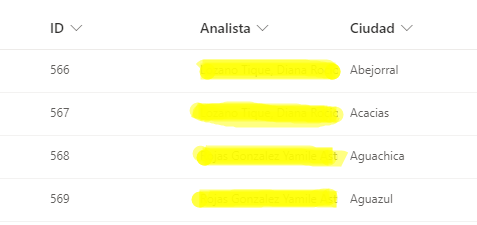
\includegraphics[scale=0.5]{Capitulo3/imagenes/8.png}
	\caption{Lista asignación analista}
	\label{Aanalista}
\end{figure}

\begin{itemize}
	\item \textbf{ID: }Es una columna numérica única autoincrementable  que define SharePoint de manera automática.
	\item \textbf{Analista: } En esta columna se almacenan valores de tipo alfanuméricos donde se guarda el nombre de distintos analistas y la ciudad o zona que tienen asignado, se definió de ``Una sola línea de texto''.
	\item \textbf{Ciudad: }Es un valor alfanumérico donde se almacena nombre de distintas ciudades o municipios, se definió de tipo ``Una sola línea de texto''.
\end{itemize}

\subsection{Forms}
En las figuras ~\ref{fig:FreporteFalla}, ~\ref{fig:CuentaCodigoDelCajero}, ~\ref{fig:CuentaCodigoDelCajero2} y ~\ref{fig:FinForm}. Se muestra el formulario donde los colaboradores del banco pueden reportar las falla de los cajeros automáticos.

\begin{figure}[H]
	\centering
	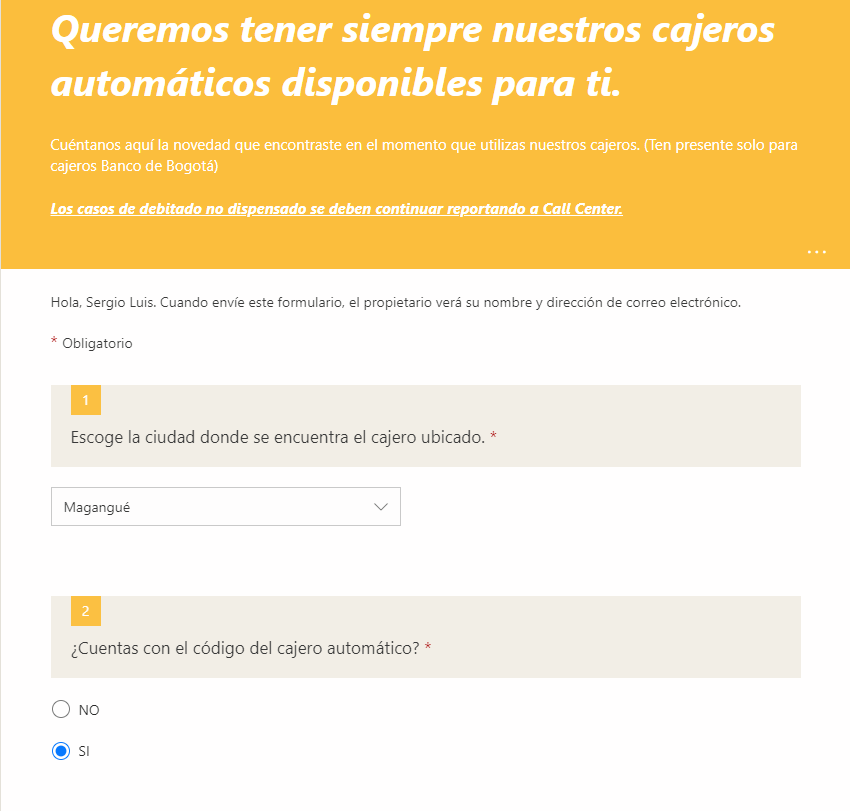
\includegraphics[scale=0.3]{Capitulo3/imagenes/f1.png}
	\caption{Formulario reporte falla cajero}
	\label{fig:FreporteFalla}
\end{figure}
\begin{figure}[H]
	\centering
	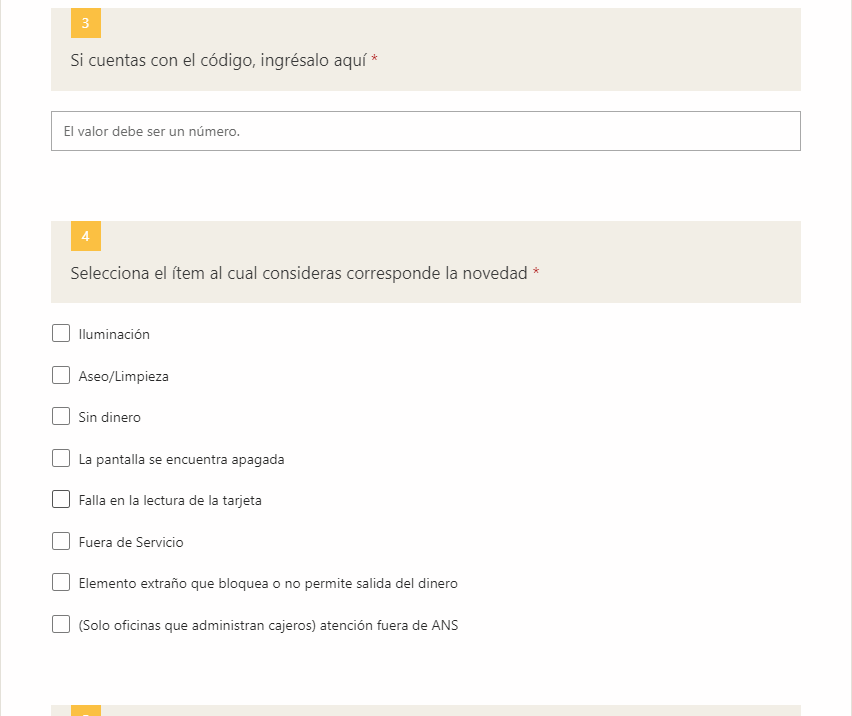
\includegraphics[scale=0.3]{Capitulo3/imagenes/f2.png}
	\caption{Cuenta con el código del cajero}
	\label{fig:CuentaCodigoDelCajero}
\end{figure}
\begin{figure}[H]
	\centering
	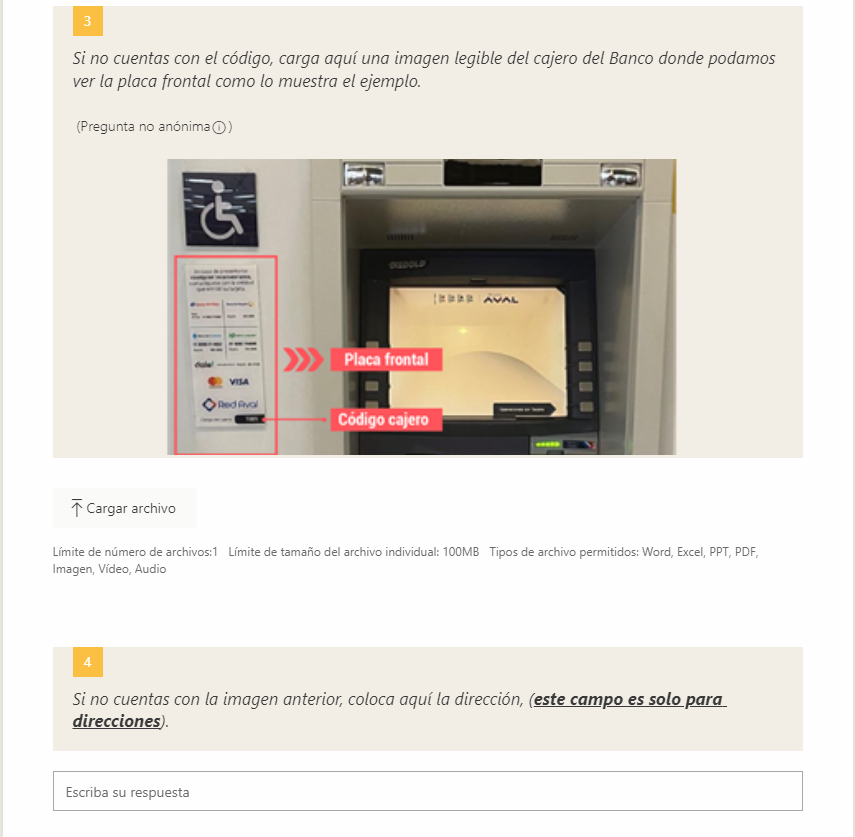
\includegraphics[scale=0.3]{Capitulo3/imagenes/f2.2.png}
	\caption{No cuenta con el código del cajero}
	\label{fig:CuentaCodigoDelCajero2}
\end{figure}
\begin{figure}[H]
	\centering
	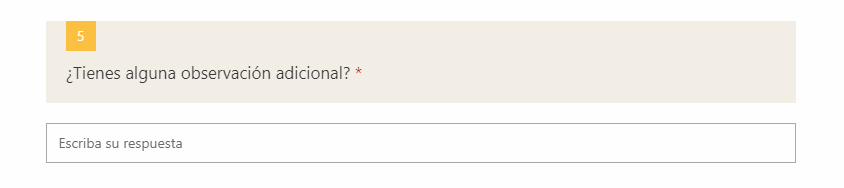
\includegraphics[scale=0.3]{Capitulo3/imagenes/f3.png}
	\caption{Fin del formulario}
	\label{fig:FinForm}
\end{figure}

\subsection{Power Automate}
\subsubsection{Flujo Administración de cajeros automáticos}
Se definió un flujo de nube automatizado que se desencadena automáticamente al recibir una nueva respuesta del formulario ``Queremos tener siempre nuestros cajeros automáticos disponibles para ti'' ~\ref{fig:DesFlu}, seguido se ejecuta la acción ``Obtener los detalles de la respuesta''.
\begin{figure}[H]
	\centering
	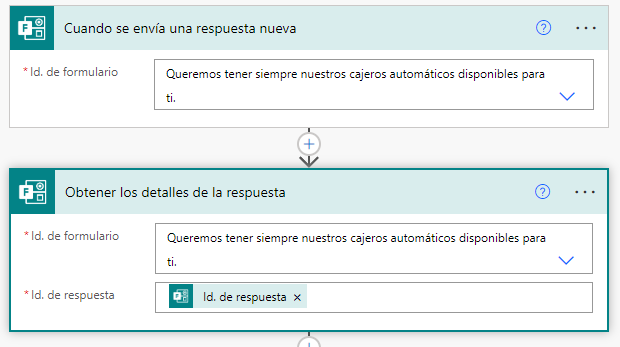
\includegraphics[scale=0.5]{Capitulo3/imagenes/flujo1.png}
	\caption{Desencadenador del flujo}
	\label{fig:DesFlu}
\end{figure}

Las siguientes cuatro acciones ~\ref{fig:DeclVar} utilizan la acción ``Inicializar variable'', se declaran cuatro variables (VarCorreoAnalista, VarIDelemento, varFalla, VarVinculelemento) todas de tipo cadena estas, variables  que se usan en pasos posteriores.
\begin{figure}[H]
	\centering
	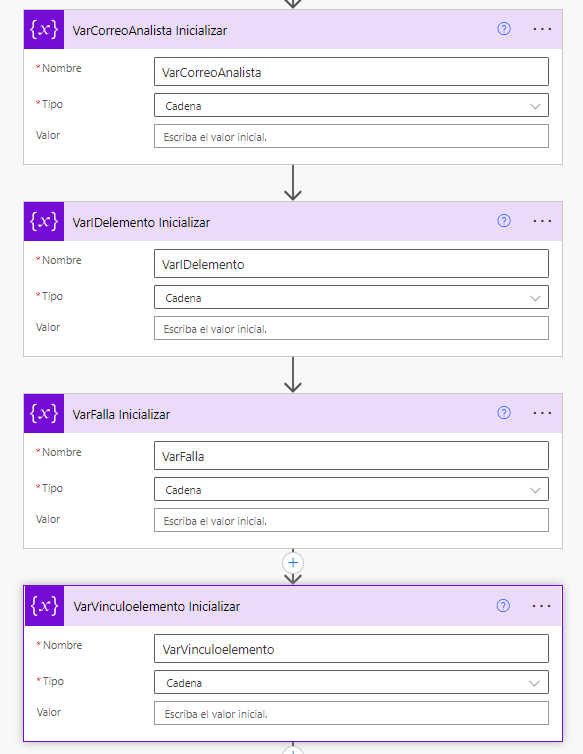
\includegraphics[scale=0.5]{Capitulo3/imagenes/flujo2.png}
	\caption{Declaración de variables}
	\label{fig:DeclVar}
\end{figure}

La siguiente acción ~\ref{fig:Consultaycondición} hace una consulta de la lista ``Asignación analista'' y trae aquellos campos que cumplan con la condición de la casilla consulta de filtro, en este caso se filtra por aquellos donde la Ciudad sea igual a la ciudad que respondieron en el formulario, luego una condición se divide el flujo en dos caminos con la respuesta de la pregunta ``¿Cuentas con el código del cajero automático?''.
\begin{figure}[H]
	\centering
	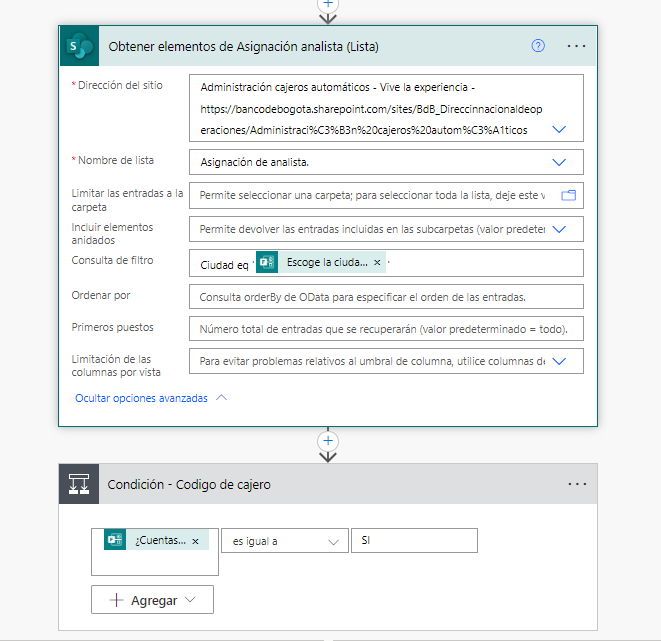
\includegraphics[scale=0.5]{Capitulo3/imagenes/flujo3.png}
	\caption{Consulta y condición}
	\label{fig:Consultaycondición}
\end{figure}

En caso de que el resultado de la condición sea verdadero, se establece la variable ``VarCorreoAnalista'' ~\ref{fig:Evar}, el cual se le asigna el ``Analista Email'' resultado de la salida de la acción ``Obtener elementos de Asignación analista (Lista)''. Se encierra en un ``aplicar a cada uno'' porque cuando se hace uso de la acción ``Obtener elemento'', una de las salidas es una lista de los elementos que coincidan con el filtro (Si se le define) y como es una lista Power Automate recorre la lista y aplica la o las acciones que contiene ``Aplicar a cada uno''.

\begin{figure}[H]
	\centering
	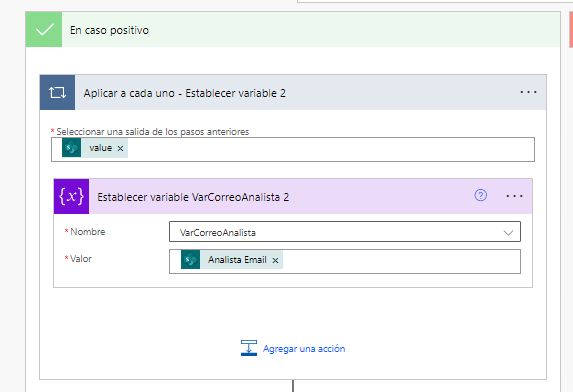
\includegraphics[scale=0.5]{Capitulo3/imagenes/flujo4.png}
	\caption{Establecer variable}
	\label{fig:Evar}
\end{figure}

El mismo caso con la acción ``Crear elemento 2'', dado que utiliza una salida (``Analista Claims'') de la acción ``Obtener elementos de Asignación analista (Lista)'' la acción se envuelve en un ``Aplicar a cada uno'' ~\ref{fig:CElemento}. La acción ``Crear elemento'' crea un nuevo elemento en la lista ``Noveades en ATM'' como parámetros de entrada, recibe la dirección del sitio de SharePoint donde se encuentra la lista y los elementos de la lista.

\begin{figure}[H]
	\centering
	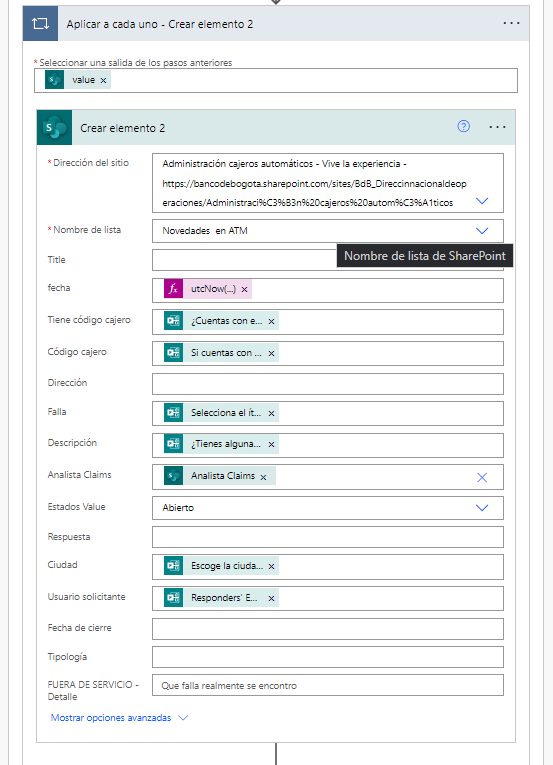
\includegraphics[scale=0.5]{Capitulo3/imagenes/flujo5.png}
	\caption{Crear elemento}
	\label{fig:CElemento}
\end{figure}

Las siguientes acciones ~\ref{fig:EVariables} son de tipo ``Establecer variable'', esta acción  asigna el valor que se quiera dar a las variables.

\begin{figure}[H]
	\centering
	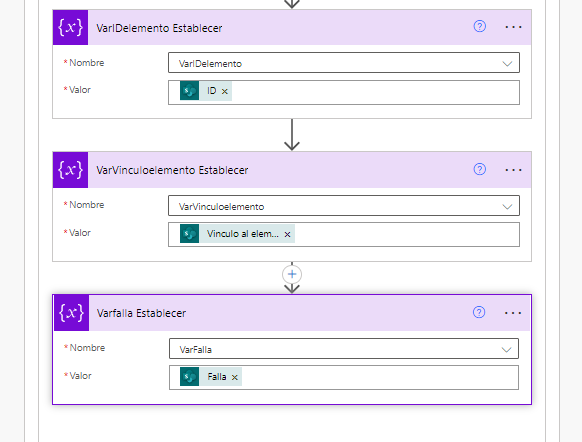
\includegraphics[scale=0.5]{Capitulo3/imagenes/flujo6.png}
	\caption{Establecer variables}
	\label{fig:EVariables}
\end{figure}

Con estas acciones acabaría el caso positivo de la condición ~\ref{fig:Cnegativo}. En el caso negativo, la primera acción que se define es una condición en la cual válida si insertaron un valor(adjunto) en la pregunta ``Si no cuentas con el código, carga aquí una imagen legible del cajero del Banco, donde podamos ver la placa frontal como lo muestra el ejemplo.'',  esta condición se hace con el fin de validar si respondieron la pregunta.

\begin{figure}[H]
	\centering
	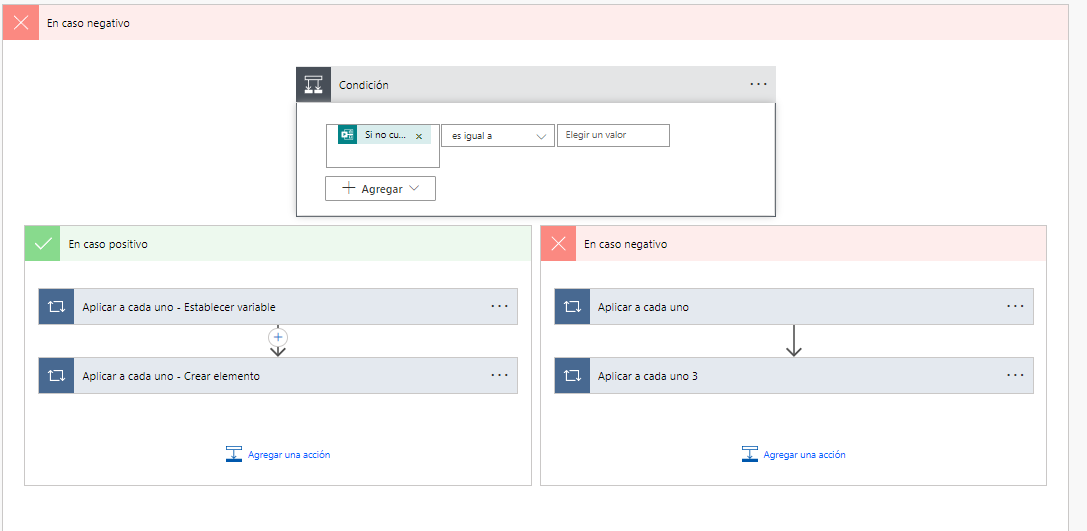
\includegraphics[scale=0.5]{Capitulo3/imagenes/flujo7.png}
	\caption{Caso negativo}
	\label{fig:Cnegativo}
\end{figure}

En el caso positivo ~\ref{fig:Evar2} las acciones a ejecutar son ``Establecer variable'', el cual está encerrado dentro de un ``Aplicar a cada uno'' dado que usa las salidas de la acción ''Obtener elementos``.

\begin{figure}[H]
	\centering
	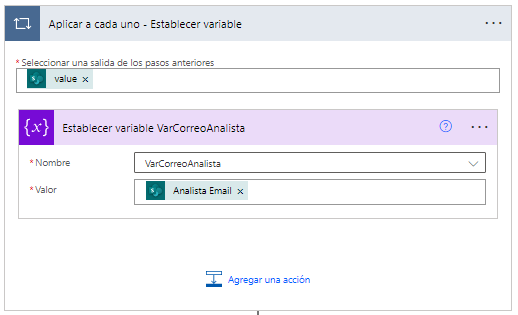
\includegraphics[scale=0.5]{Capitulo3/imagenes/flujo9.png}
	\caption{Establecer variable}
	\label{fig:Evar2}
\end{figure}

La siguiente acción `\ref{fig:Cele} es un ``crear elemento'' y dado que se usan salidas de la acción ``Obtener elementos'' se encierra dentro de un ``Aplicar a cada uno'' y se le pasan los parámetros correspondientes.

\begin{figure}[H]
	\centering
	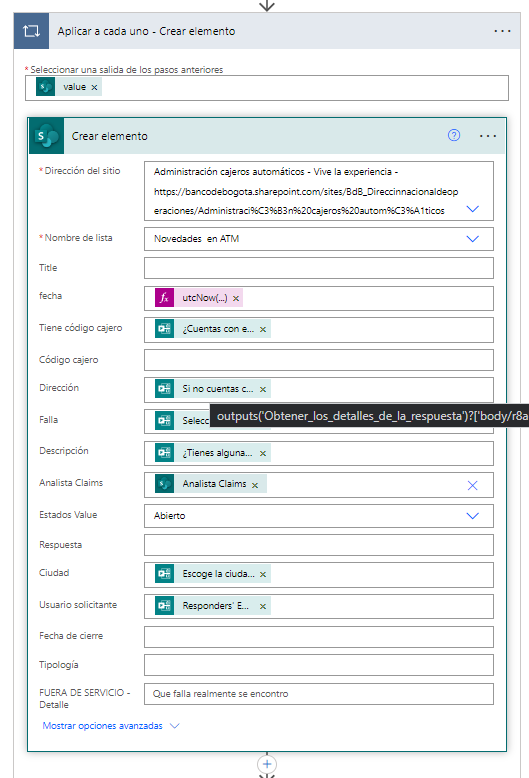
\includegraphics[scale=0.5]{Capitulo3/imagenes/flujo10.png}
	\caption{Crear elemento}
	\label{fig:Cele}
\end{figure}

Cuando se adjunta un archivo a un formulario o encuesta, este guarda la información en la nube, y descompone el archivo en su contenido y nombre. La información la guarda en un JSON y se usa la acción ``Análisis del archivo JSON'' ~\ref{fig:Cele2}el cual recibe como entrada el archivo adjunto y devuelve los elementos del JSON. Donde ``driveId'' en conjunto con ``id'' forman un id único de cada archivo y por el cual el flujo lo puede identificar.
\\
La acción ``Obtener contenido de archivo'' es una acción que recibe como parámetro de entrada la identificación del archivo o la ruta donde este se encuentra ubicado, y como salida genera el archivo codificado en base64. La acción ``Agregar datos adjuntos'' Recibe como parámetros la dirección del sitio, el nombre de la lista, el identificador del elemento al que se quiere adjuntar los datos, un nombre que es una de las salidas que genera ``Análisis del archivo JSON'' y contenido del archivo que se le pasa de la salida que genera la acción ``Obtener contenido de archivo''.

\begin{figure}[H]
	\centering
	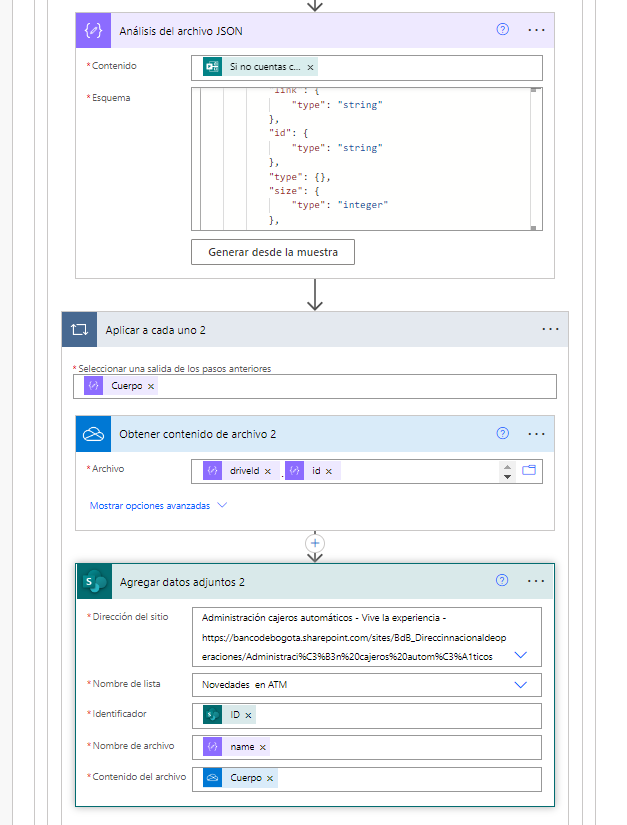
\includegraphics[scale=0.5]{Capitulo3/imagenes/flujo11.png}
	\caption{Adjuntar archivos en Sharepoint}
	\label{fig:Cele2}
\end{figure}

Las siguientes tres ~\ref{fig:defvar} acciones definen algunas variables que se inicializaron previamente, en este caso ``VarIDelemento'' variable en la que se almacena el id único que generan las listas de SharePoint, ``VarVinculoelemento'' se almacena un vínculo el cual lleva al elemento específico en la lista, ``VarFalla'' almacena la falla de la lista ``Novedades en ATM''.  Y con esto finaliza el caso positivo.

\begin{figure}[H]
	\centering
	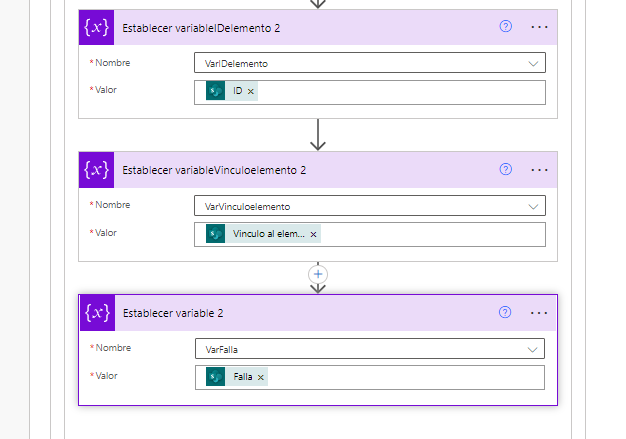
\includegraphics[scale=0.5]{Capitulo3/imagenes/flujo12.png}
	\caption{Definición de variables}
	\label{fig:defvar}
\end{figure}

En el caso negativo solo se crea el elemento con la dirección que diligencie en el formulario.

\begin{figure}[H]
	\centering
	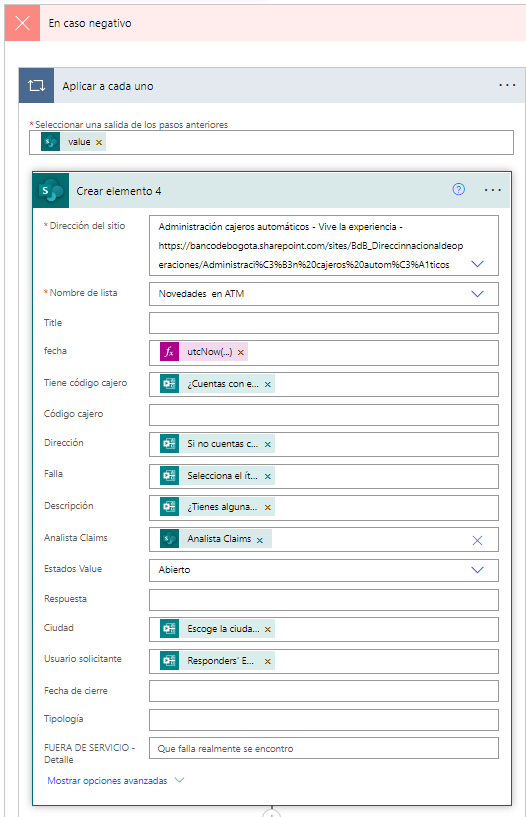
\includegraphics[scale=0.5]{Capitulo3/imagenes/flujo13.png}
	\caption{Crear elemento}
	\label{cele}
\end{figure}

Las siguientes cuatro ~\ref{fig:defvar2} acciones definen algunas variables que se habían inicializado previamente, en este caso ``VarIDelemento'' variable en la que se almacena el id único que generan las listas de SharePoint, ``VarVinculoelemento'' se almacena un vínculo el cual lleva al elemento específico en la lista, ``VarFalla'' almacena la falla de la lista ``Novedades en ATM'', ``VarCorreoAnalista'' donde se almacena el correo del analista encargado de dar solución al caso.

\begin{figure}[H]
	\centering
	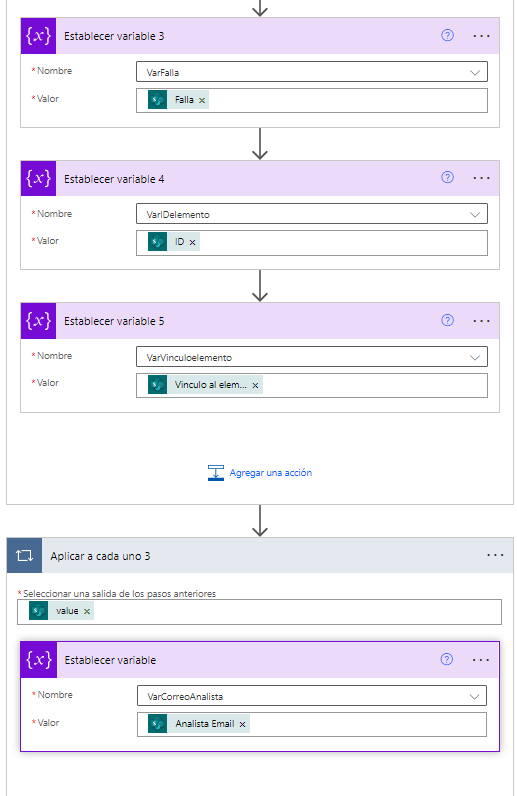
\includegraphics[scale=0.5]{Capitulo3/imagenes/flujo14.png}
	\caption{Definición de variables}
	\label{fig:defvar2}
\end{figure}

Las siguientes dos acciones de Outlook son acciones las cuales reciben como parámetro a quien va dirigido el correo (usuario que envió el formulario en la primera y VarCorreoAnalista), el asunto en la primera acción se define como un texto fijo ``Solicitud creada ID: '' y dos variables ``VarIDelemento'' y ``VarFall'', en la segunda acción el texto fijo es ``Solicitud radicada ID: '' y complementan con el id del elemento (VarIDelemento) y la falla(VarFalla).
\\

El cuerpo en la primera acción es un texto fijo con el cual se notifica al colaborador que recibió la solicitud, y el cuerpo de la segunda acción notifica al analista que ha radicado una solicitud y se le envía la variable ``VarVinculoelemento''.

\begin{figure}[H]
	\centering
	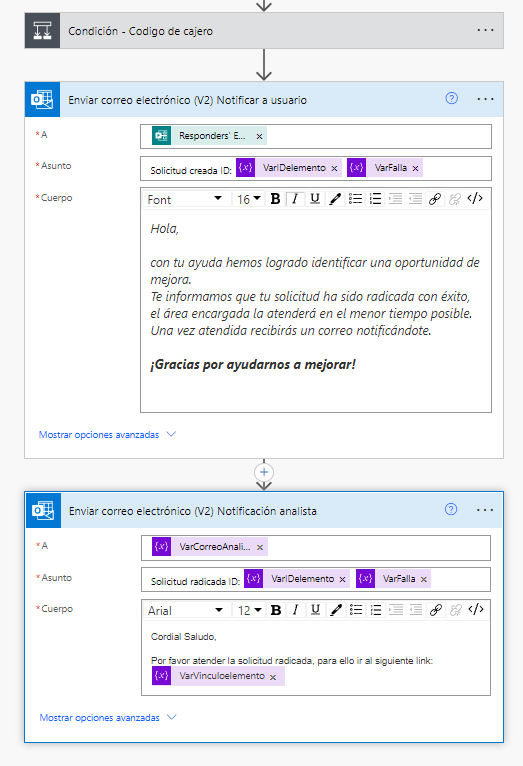
\includegraphics[scale=0.5]{Capitulo3/imagenes/flujo15.png}
	\caption{Notificaciones}
	\label{not}
\end{figure}


\subsubsection{Notificación de respuesta}
Es un flujo ~\ref{fig:not2} más sencillo, ya que tiene como desencadenador ``Cuando se cree o modifica un elemento'' de la lista ``Novedades en ATM'', el flujo se desencadenará siempre que se cree o modifique en la lista, la acción siguiente es una condición en la que se verifica que el campo ``Respuesta'' de la lista ``Novedades en ATM'' no sea igual a ``Null'' o esté vacío y su estado sea igual a ``Atendido'', con solo una acción el caso positivo.
Cuando esa condición es cierta significa que el analista modificó el campo ``Respuesta'' y cambió el estado a ``Atendido''. Se envía un correo al usuario que hizo la solicitud notificándole que fue atendida, enviándole el ID de la solución y la ``Respuesta'' que haya dado el analista.

\begin{figure}[H]
	\centering
	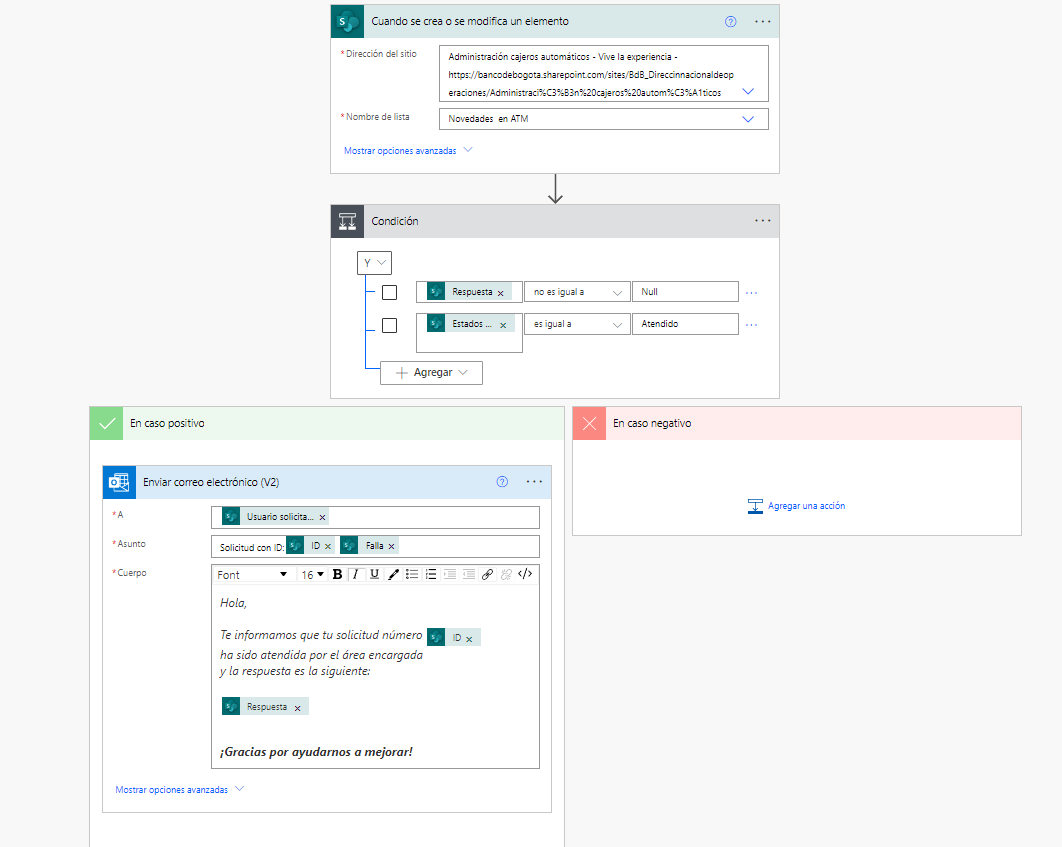
\includegraphics[scale=0.5]{Capitulo3/imagenes/flujo16.png}
	\caption{Notificación usuario}
	\label{fig:not2}
\end{figure}